\section{introduction}

%文本输入是平板电脑上的刚性需求,用户使用触屏软键盘来完成各种文本输入任务如搜索、办公。然而,触屏软键盘在输入效率(vs)、疲劳程度[xx]和视觉注意力负担[xx]等诸多方面上都比不上物理键盘。用户可以将手指休息在物理键盘上,却不能将手指休息在触屏键盘上,因为触屏键盘上的休息行为会导致误识别。这一点不同给物理键盘带来了两大优势:一是减轻了疲劳,保证了用户高效输入的持续性[xx];二是用户可以通过触摸按键纹理来对齐他们的手指,从而实现盲打,大幅度提高输入效率[xx]。为了弥补物理键盘和软键盘之间的GAP,我们提出了TypeBoard,一款带有防误触功能的触屏软键盘,它允许用户将手指休息在触屏键盘上。TypeBoard的一个直观的好处是减低疲劳。更进一步,在TypeBoard算法的帮助下,我们有机会通过添加膜层[xx]或可变形触屏[xx]等方案给软键盘添加触觉纹理,从而在软键盘上支持盲打,提高输入效率。

Increasingly more people are using tablets for text input tasks such as searching the Internet, writing email messages, and office work \cite{2018-Japanese}. They use software keyboards on the touchscreens of the tablets. However, there is a gap between the tablet keyboard and the physical keyboard in aspects of the fatigue problem \cite{2014-Differences}, switching of visual attention \cite{2017-BlindType, 2010-NoLook, 2010-Eyes}, and typing speed \cite{1991-Improving, 2011-Typing}. Users can rest their fingers on the physical keyboard but cannot rest on the tablet keyboard because touching the screen causes misrecognition. The resting behavior plays an important role in the usability of physical keyboards. First, it reduces fatigue \cite{2013-TapBoard}. Second, users align their fingers by touching the keys and achieve touch typing \cite{2010-Warning, 1995-Use, 2011-Hierarchical, 2015-Haptic}. Touch typists type quickly because they do not use the sense of sight to find the keys. To bridge the gap between tablet keyboard and the physical keyboards, we proposed TypeBoard, a software keyboard that prevents unintentional touch. As figure \ref{fig:teaser} shows, the TypeBoard allows users to rest their fingers on the touchscreen. The TypeBoard prevents unintentional touches such as fingers resting and thenar eminence touches while passing users' typing behaviors. Furthermore, if we provide tactile landmarks on the TypeBoard through deformable screens \cite{Website-Tactus}, and changeable surface texture \cite{2011-Stimtac, 2010-TeslaTouch, 2011-Enhancing}, the TypeBoard can support touch typing.

% (e.g., 38 WPM on iPad vs. 69 WPM on MacBook \cite{2010-Keyboard})
% TypeBoard prevents unintentional touches such as fingers resting and thenar eminence touches while passing users' typing behaviors.

\begin{figure}[!htbp]
	\centering
	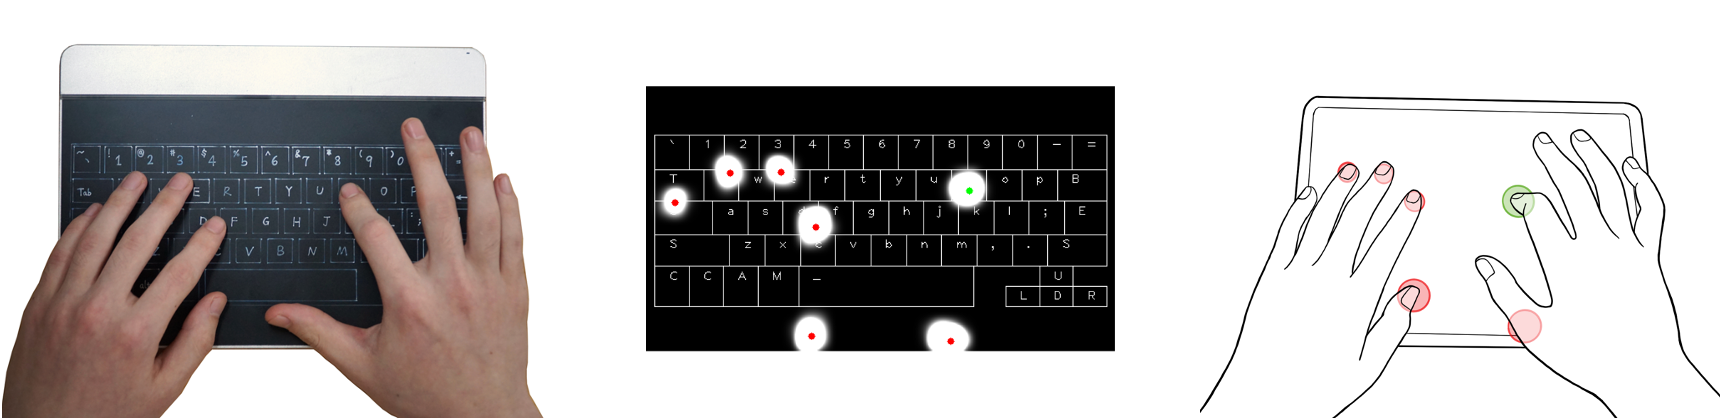
\includegraphics[width=\textwidth]{figures/teaser.png}
	\caption{The TypeBoard is a software keyboard that prevent unintentional touch such as fingers resting and thenar eminence touches. }
	\label{fig:teaser}
\end{figure}{}

%Previous work has demonstrated the feasibility of providing tactile landmarks on touchscreens through deformable screens \cite{Website-Tactus} and changeable surface texture \cite{2011-Stimtac, 2010-TeslaTouch, 2011-Enhancing}. Under this premise, the TypeBoard with tactile landmarks is expected to support touch typing on the touchscreen.

%在触屏键盘上区分打字点击和“误触”并不是我们的首创。在2013年,TapBoard就曾经提出将Tapping动作看作打字点击,而将其它触摸事件视为误触。Tapping的定义是“触摸时间低于xx毫秒,位移低于xx毫米的点击”。用户需要主动去适应TapBoard的技术方案,这影响了用户输入的自然性和舒适性,同时这种基于阈值的方法识别准确率也不高(xx.x\%)。为了克服TapBoard的局限性,这份工作从用户的角度出发,将打字点击定义为“表达键入意图的点击”。在此前提下,我们通过用户实验来收集数据,探索用户的打字行为,再根据用户行为设计TypeBoard防误触算法。

We are not the first to explore the detection of unintentional touch on the touchscreen keyboard. In 2013, Kim et al. proposed TapBoard \cite{2013-TapBoard}, a touchscreen keyboard that regards tapping actions as keystrokes and the other touches as unintentional touches. Tapping actions were those touches that neither exceed a timeout threshold of 450 ms nor exceed a displacement threshold of 15 mm. Users adapted to the thresholds, which led to unnatural typing behavior. TapBoard cannot judge the intention of touch until the touch is released. Even so, the accuracy is only 97\%. We have two strategies to overcome TapBoard's limitations of naturalness and recognition performance. First, to ensure natural interaction, we defined \emph{unintentional touches} as those touches that do not intend to input words. Second, we conducted user studies to understand user behavior, based on which we designed the algorithm of TypeBoard.

Techniques change user behavior. For example, users will not rest their fingers on the tablet keyboard unless the touchscreen prevents unintentional touches. Thus, to design TypeBoard, it is valuable to understand the users' typing behavior on the TypeBoard itself. However, how can we observe the user behavior on the TypeBoard before we have developed the TypeBoard? To solve this "chicken and egg" problem, we followed an iterative process, i.e., we developed a semi-finished TypeBoard, then analyze the user behavior on it, and finally improved the technique by using the latest dataset. In details, we conducted three user studies, each contributing to answering one of the three research questions as follows:

%然而,“探索用户在TypeBoard上的打字行为”是困难的,因为用户的行为会受到防误触算法的能力的影响。例如,用户在防误触软键盘上打字时,可能会将手指休息在触屏上,带来更多对识别有挑战性的误触点。这是一个蛋鸡悖论,即我们如何在设计出防误触触屏键盘之前,探索用户在防误触键盘上的打字行为呢?为了解决这一问题,我们采用了迭代的方案。我们共组织了三个用户实验,分别回答了以下三个研究问题:

\begin{enumerate}
	\item{\textbf{RQ1):} \emph{What is the user behavior on an imaginary TypeBoard?} We conducted study one to collect users' typing data on a touchpad that has no feedback. Participants could not input words, instead, they pretended to input words, and imagined that the touchpad prevents unintentional touch. We found eleven categories of unintentional touches. The three most common ones were multiple finger resting, hypothenar eminence touches, and repeated touch reporting. We developed a semi-finished TypeBoard based on the analysis of user behavior.}
	\item{\textbf{RQ2):} \emph{What is the user behavior on the TypeBoard?} We conducted study two to collect users' typing data on the (semi-finished) TypeBoard. We did not found new unintentional touch behavior. However, the user behavior in study two was different from study one in details. For example, the average force of intentional touch was 33.78\% lighter in study two because users learned that they could type without much effort, gradually making the touch lighter. We used the data in study two to improve the TypeBoard, achieving an accuracy of 98.88\%, with a delay of 100 ms.}
	\item{\textbf{RQ3):} \emph{What is the performance of the TypeBoard? What if there are tactile landmarks on the TypeBoard?} We conducted study three to evaluate users' typing performance on three settings, including ordinary tablet keyboard, TypeBoard, and TypeBoard plus (the TypeBoard with tactile landmarks). The result shows that the TypeBoard improves the efficiency and usability of touchscreen typing from many aspects, including avoiding fatigue, relieving cognitive load, and reducing error rates. The TypeBoard plus further improves the performance of the TypeBoard by allowing touch typing on the tablet.}
\end{enumerate}

The contribution of this work is three-fold. First, we proposed TypeBoard, which identifies unintentional touch in text input tasks with high accuracy (98.88\%) and low latency (100 ms). Second, we explored the user behavior on the touchscreen keyboard with unintentional touch prevention. We published the dataset. Third, we empirically demonstrated the advantages of the TypeBoard in typing speed, error rate and subjective user experience.
